\documentclass[11pt]{article}
\usepackage[utf8]{inputenc}
%\usepackage[brazil]{babel}
\usepackage{palatino}
\usepackage{fullpage}
\usepackage{hyperref}

\usepackage{multicol}
\usepackage{graphicx}
\usepackage{float}
\usepackage{moreverb}
\usepackage{verbatim}

\usepackage{multirow}

\title{\textbf{AMI and HDB1 Line Codes - VHDL Implementation.}}
\author{Ribamar Santarosa, ribamar@gmail.com}
\date{Outubro/Novembro 2006.}

\begin{document}
\maketitle 


\begin{abstract}
Line codings are methods for coding digital data for making them 
less susceptible to signal losses during transmission. This project 
implements the AMI --- Alternate Mark Inverse --- and HDB1 --- High
Density Bipolar of order 1 codings. This file documents their
implementation. 
\end{abstract}

\section{Specification.}


\paragraph{AMI.} This coding takes a binary sequency into a
ternary sequency having the signals 0, +1, -1 by the following way: 

\begin{itemize}
\item Inputs of 1 are coded as +1 or -1 alternately.
\item Inputs of 0 are coded always as 0. 
\end{itemize}

Example: 
\begin{verbatim}
Input 
 1 0  1 0  1  1 0 0 0  1 0  1  1 0 0  1 0  1 0 0 0  1  1  1
Output
+1 0 -1 0 +1 -1 0 0 0 +1 0 -1 +1 0 0 -1 0 +1 0 0 0 -1 +1 -1
\end{verbatim}

\paragraph{HDB1.} This coding takes a binary sequency into a 
ternary sequency having the signals 0, +1, -1 by the following way:

\begin{itemize}
\item Inputs of 1 are coded as either +1 or -1.
\item Paired inputs of 0 are coded as either +1+1 or -1-1.   
\item Isolated inputs of 0, ie, inputs of 0 not followed by 1 which
weren't paired to another 0 (thus forming +1+1 or -1-1) are coded 
as 0. 
\item Outputs have always alternate signals. If the last output was
-1 and the input is 00, the next output is coded as +1+1, if the
last output was -1-1 and the input is 1, the next output is +1. 
\end{itemize}

Example: 
\begin{verbatim}
Input 
 1 0  1 0  1  1  0  0 0  1 0  1  1  0  0  1 0  1  0  0  0  0  1  1
Output
+1 0 -1 0 +1 -1 +1 +1 0 -1 0 +1 -1 +1 +1 -1 0 +1 -1 -1 +1 +1 -1 +1
\end{verbatim}



%\begin{multicols}{2}

\section{AMI Encoder. }

\begin{figure}[H]
\centering
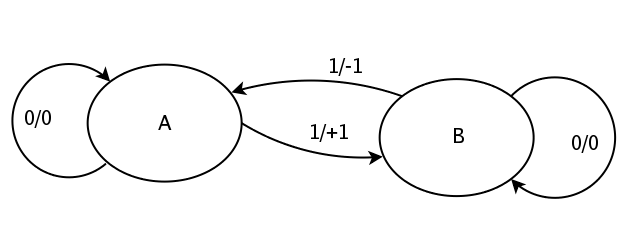
\includegraphics[scale=0.35]{estados-ami_enc}
\caption[ ]{\label{estados-ami_enc} State Map.  }
\end{figure}

\begin{multicols}{2}
Truth Table: \\

\begin{tabular}{|c|c|cc|c|}
\hline
$q$ & $e$ & $S_0$ & $ S_1$ & $q^+$ \\
\hline
0 & 0 & 0 & 0 & 0 \\
0 & 1 & 1 & 0 & 1 \\
\hline
1 & 0 & 0 & 0 & 1 \\
1 & 1 & 0 & 1 & 0 \\
\hline
\end{tabular}

Karnaugh Map isn't necessary: \\
$ S_0 = e \cdot q'$ \\
$ S_1 = e \cdot q $ \\
$ q^+ = e \oplus q$ \\

\end{multicols}

%\hrule

\section{AMI Decoder. }
\begin{multicols}{2}


\begin{figure}[H]
\centering
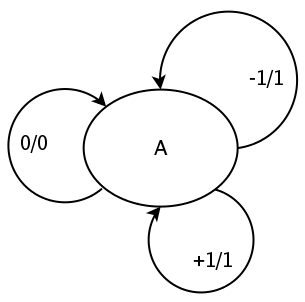
\includegraphics[scale=0.35]{estados-ami_dec}
\caption[ ]{\label{estados-ami_dec} State Map. }
\end{figure}


Truth Table: 

\begin{tabular}{|cc|c|}
\hline
$e_0$ & $e_1$ & $S$  \\
\hline
0 & 0 & 0 \\
0 & 1 & 1 \\
1 & 0 & 1 \\
1 & 1 & $X$ \\
\hline
\end{tabular}

\vspace{50pt}
Karnaugh Map isn't necessary: \\
$ S = e_0 + e_1 $ \\

\end{multicols}
%\hrule


\section{HDB1 Encoder. }
\begin{figure}[H]
\centering
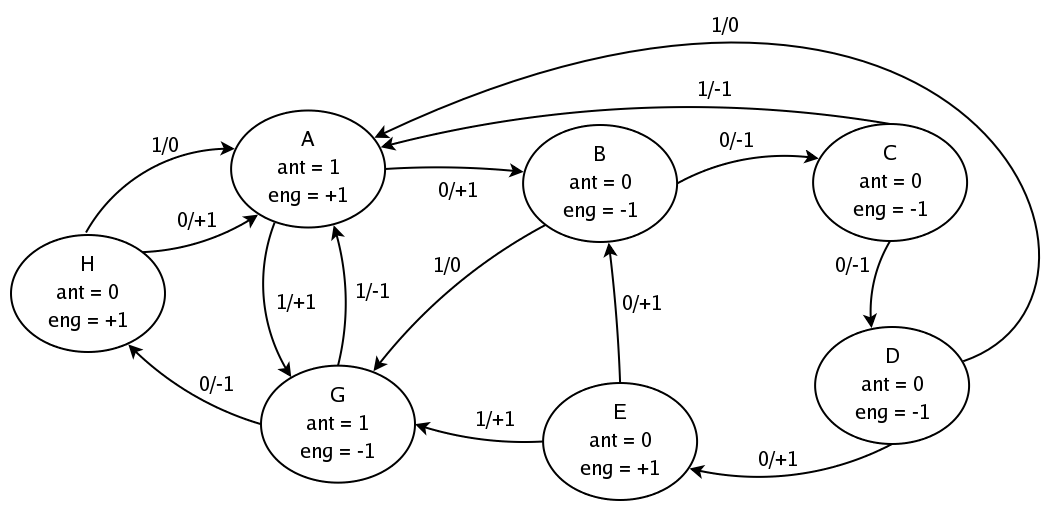
\includegraphics[scale=0.35]{estados-hdb1_enc}
\caption[ ]{\label{estados-hdb1_enc} State Map. }
\end{figure}


\begin{multicols}{2}


Truth Table: \\
 ~\\
\begin{tabular}{|cccc|ccc|cc|}
\hline
$E$ & $q_0$ & $q_1$ & $q_2$ & $q_0^+$ & $q_1^+$ & $q_2^+$ & $S_0$ & $S_1$ \\
\hline
$0$ & $0$ & $0$ & $0$ &    $0$ & $0$ & $1$ &    $1$ & $0$  \\
$1$ & $0$ & $0$ & $0$ &    $1$ & $1$ & $0$ &    $1$ & $0$  \\
\hline
$0$ & $0$ & $0$ & $1$ &    $0$ & $1$ & $0$ &    $0$ & $1$  \\
$1$ & $0$ & $0$ & $1$ &    $1$ & $1$ & $0$ &    $0$ & $0$  \\
\hline
$0$ & $0$ & $1$ & $0$ &    $0$ & $1$ & $1$ &    $0$ & $1$  \\
$1$ & $0$ & $1$ & $0$ &    $0$ & $0$ & $0$ &    $0$ & $1$  \\
\hline
$0$ & $0$ & $1$ & $1$ &    $1$ & $0$ & $0$ &    $1$ & $0$  \\
$1$ & $0$ & $1$ & $1$ &    $0$ & $0$ & $0$ &    $0$ & $0$  \\
\hline
$0$ & $1$ & $0$ & $0$ &    $0$ & $0$ & $1$ &    $1$ & $0$  \\
$1$ & $1$ & $0$ & $0$ &    $1$ & $1$ & $0$ &    $1$ & $0$  \\
\hline
$$X$$ & $1$ & $0$ & $1$ &    $$X$$ & $$X$$ & $$X$$ &    $$X$$ & $$X$$  \\
\hline
$0$ & $1$ & $1$ & $0$ &    $1$ & $1$ & $1$ &    $0$ & $1$  \\
$1$ & $1$ & $1$ & $0$ &    $0$ & $0$ & $0$ &    $0$ & $1$  \\
\hline
$0$ & $1$ & $1$ & $1$ &    $0$ & $0$ & $0$ &    $1$ & $0$  \\
$1$ & $1$ & $1$ & $1$ &    $0$ & $0$ & $0$ &    $0$ & $1$  \\
\hline
\end{tabular}

$q_0^+$:
\begin{tabular}{|cc|c|c|c|c|}
\hline
\multicolumn{6}{|c|}{$E q_0$ } \\
           & & \tiny{$00$} & \tiny{$01$}  & \tiny{$11$}  & \tiny{$10$}  \\
           & \tiny{$00$} &   &   & 1 & 1 \\
$q_1 q_2$  & \tiny{$01$} &   & $X$ & $X$ & 1 \\
           & \tiny{$11$} & 1 &   &   &   \\
           & \tiny{$10$} &   & 1 &   &   \\
\hline
\end{tabular}

$q_0^+ = E . q_1' + E'.q_0'.q_1.q_2 + E'.q_0.q_1 . q_2' $

$q_1^+$:
\begin{tabular}{|cc|c|c|c|c|}
\hline
\multicolumn{6}{|c|}{$E q_0$ } \\
           & & \tiny{$00$} & \tiny{$01$}  & \tiny{$11$}  & \tiny{$10$}  \\
           & \tiny{$00$} &   &   & 1 & 1 \\
$q_1 q_2$  & \tiny{$01$} & 1 & $X$ & $X$ & 1 \\
           & \tiny{$11$} &   &   &   &   \\
           & \tiny{$10$} & 1 & 1 &   &   \\
\hline
\end{tabular}

$q_1^+ = E . q_1' + q_1'.q_2 + E'.q_1.q_2' $

$q_2^+$:
\begin{tabular}{|cc|c|c|c|c|}
\hline
\multicolumn{6}{|c|}{$E q_0$ } \\
           & & \tiny{$00$} & \tiny{$01$}  & \tiny{$11$}  & \tiny{$10$}  \\
           & \tiny{$00$} & 1 & 1 &   &   \\
$q_1 q_2$  & \tiny{$01$} &   & $X$ & $X$ &   \\
           & \tiny{$11$} &   &   &   &   \\
           & \tiny{$10$} & 1 & 1 &   &   \\
\hline
\end{tabular}

$q_2^+ = E'. q_2'$

$S_0$: 
\begin{tabular}{|cc|c|c|c|c|}
\hline
\multicolumn{6}{|c|}{$E q_0$ } \\
           & & \tiny{$00$} & \tiny{$01$}  & \tiny{$11$}  & \tiny{$10$}  \\
           & \tiny{$00$} & 1 & 1 & 1 & 1 \\
$q_1 q_2$  & \tiny{$01$} &   & $X$ & $X$ &   \\
           & \tiny{$11$} & 1 & 1 &   &   \\
           & \tiny{$10$} &   &   &   &   \\
\hline
\end{tabular}

$S_0 = q_1'. q_2' + E'.q_1. q_2 $

$S_1$: 
\begin{tabular}{|cc|c|c|c|c|}
\hline
\multicolumn{6}{|c|}{$E q_0$ } \\
           & & \tiny{$00$} & \tiny{$01$}  & \tiny{$11$}  & \tiny{$10$}  \\
           & \tiny{$00$} &   &   &   &   \\
$q_1 q_2$  & \tiny{$01$} & 1 & $X$ & $X$ &   \\
           & \tiny{$11$} &   &   &   &   \\
           & \tiny{$10$} & 1 & 1 & 1 & 1 \\
\hline
\end{tabular}

$S_1 = q_1. q_2' + E'.q_1'. q_2 $


\end{multicols}

\vspace{10pt}
%\hrule

\section{HDB1 Decoder. }

\begin{figure}[H]
\centering
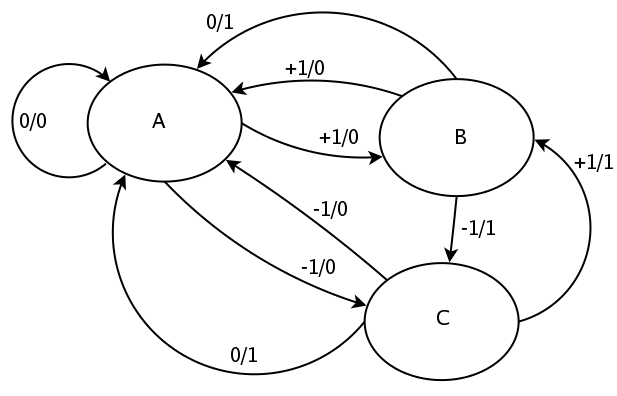
\includegraphics[scale=0.2665]{estados-hdb1_dec}
\caption[ ]{\label{estados-hdb1_dec} State Map. }
\end{figure}


\begin{multicols}{2}

Truth Table: 
\begin{tabular}{|cc|cc|cc|c|}
\hline
$e_1$ & $e_0$ & $q_1$ & $q_0$ & $q^+_0$ & $q^+_1$ & $S$ \\
\hline
0 & 0 & 0 & 0   & 0 & 0 & 0 \\
0 & 0 & 0 & 1   & 0 & 0 & 1 \\
0 & 0 & 1 & 0   & 0 & 0 & 1 \\
0 & 0 & 1 & 1   & $X$ & $X$ & $X$ \\
\hline
0 & 1 & 0 & 0   & 0 & 1 & 0 \\
0 & 1 & 0 & 1   & 0 & 0 & 0 \\
0 & 1 & 1 & 0   & 0 & 1 & 1 \\
0 & 1 & 1 & 1   & $X$ & $X$ & $X$ \\
\hline
1 & 0 & 0 & 0   & 0 & 1 & 0 \\
1 & 0 & 0 & 1   & 1 & 0 & 1 \\
1 & 0 & 1 & 0   & 0 & 0 & 0 \\
1 & 0 & 1 & 1   & $X$ & $X$ & $X$ \\
\hline
1 & 1 & 0 & 0   & $X$ & $X$ & $X$ \\
1 & 1 & 0 & 1   & $X$ & $X$ & $X$ \\
1 & 1 & 1 & 0   & $X$ & $X$ & $X$ \\  
1 & 1 & 1 & 1   & $X$ & $X$ & $X$ \\
\hline
\end{tabular}

$q0$: 
\begin{tabular}{|cc|c|c|c|c|}
\hline
\multicolumn{6}{|c|}{$q_1 q_0$ } \\
           & & \tiny{$00$} & \tiny{$01$}  & \tiny{$11$}  & \tiny{$10$}  \\
           & \tiny{$00$} &   &   & $X$ &   \\
$e_0 e_1$  & \tiny{$01$} &   &   & $X$ &   \\
           & \tiny{$11$} & $X$ & $X$ & $X$ & $X$ \\
           & \tiny{$10$} &   & 1 & $X$ &   \\
\hline
\end{tabular}

$q_0^+ = q_0'. e_0$

$q1$: 
\begin{tabular}{|cc|c|c|c|c|}
\hline
\multicolumn{6}{|c|}{$q_1 q_0$ } \\
           & & \tiny{$00$} & \tiny{$01$}  & \tiny{$11$}  & \tiny{$10$}  \\
           & \tiny{$00$} &   &   & $X$ &   \\
$e_0 e_1$  & \tiny{$01$} & 1 &   & $X$ & 1 \\
           & \tiny{$11$} & $X$ & $X$ & $X$ & $X$ \\
           & \tiny{$10$} & 1 &   & $X$ &   \\
\hline
\end{tabular}


$q_1^+ = q_1'. e_1$

$S$: 
\begin{tabular}{|cc|c|c|c|c|}
\hline
\multicolumn{6}{|c|}{$q_1 q_0 $ } \\
           & & \tiny{$00$} & \tiny{$01$}  & \tiny{$11$}  & \tiny{$10$}  \\
           & \tiny{$00$} &   & 1 & $X$ & 1 \\
$e_1 e_2$  & \tiny{$01$} &   &   & $X$ & 1 \\
           & \tiny{$11$} & $X$ & $X$ & $X$ & $X$ \\
           & \tiny{$10$} &   & 1 & $X$ &   \\
\hline
\end{tabular}

$ S = q_0. e_0' + q_1. e_1' $


\vspace{10pt}

\end{multicols}

%\hrule


\end{document}

